	
%In this work, our aim is to investigate how formal methods can be applied in the context of mobile robot algorithms.

Les tâches qui peuvent être effectuées par des robots autonomes sont
de plus en plus nombreuses et complexes, à la fois dans notre vie de
tous les jours et dans l'industrie.  De nombreuses études se sont
intéressées récemment aux réseaux de robots mobiles et autonomes qui
doivent coopérer pour réaliser une tâche complexe commune qu'ils ne
peuvent accomplir seuls. 
% Ces travaux peuvent être trouvés par exemple
On peut trouver des exemples de tels travaux
dans~\cite{Prencipe13, butucaru_distributed_2011,FPS12}.  Les
applications 
%dans lesquelles de tels systèmes sont utilisés
concernées par ce type de systèmes
comprennent l'exploration d'environnements inconnus, la surveillance
de zones à risque, la construction de cartes pour de telles zones,
etc. Par exemple, ces robots peuvent patrouiller les quais dans un
port, comme décrit dans la Figure~\ref{fig:port:resume}.
\begin{figure}[h]
\begin{tikzpicture}[x=1em,y=1em,fill=blue!50]
  \pgfmatrix{rectangle}{center}{mymatrix}
    {\pgfusepath{}}{\pgfpointorigin}{}
    {
	\node[] at (0,0) {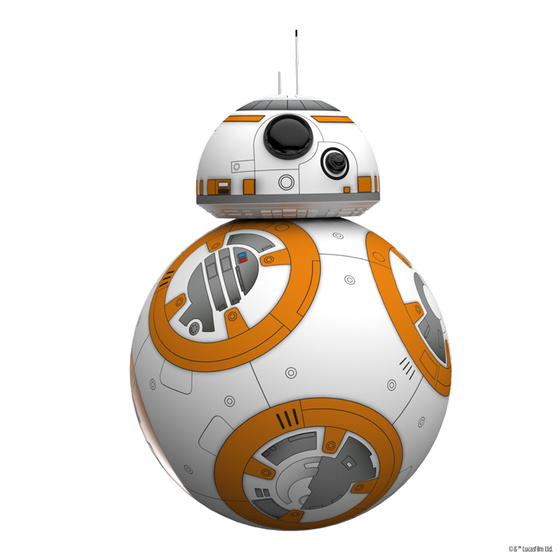
\includegraphics[scale=0.06]{robot}};
      \fill (1,-4)  rectangle (2,1);
      \fill (2,-3)  rectangle (3,0);%\atorig
	 \pgfmatrixnextcell
      \fill (-3,0)  rectangle (1,1);%\atorig2 
	 \pgfmatrixnextcell
      \fill (-1,-4) rectangle (0,-1);%\atorig3 
	 \pgfmatrixnextcell
      \fill (0,-1) rectangle (-1,-3);%\atorig4 
	 \pgfmatrixnextcell %ici pour un carré
      \fill (4,-3) rectangle (5,1);
      \fill (1,3.5) rectangle (6,2.5); 
      \fill (-1,0.5)  rectangle (4,1.5);%\atorig5
      \fill (3,-1) rectangle (4,-3);
	  \pgfmatrixnextcell 
	 \node[] at (-3,2) {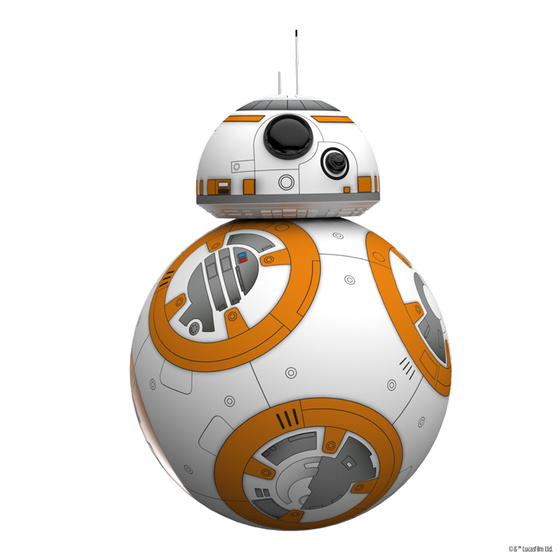
\includegraphics[scale=0.06]{robot}};
      \fill (0,-1)  rectangle (2,0);%\atorig6 
      \fill (-2,-2) rectangle (0,-1);
	  \pgfmatrixnextcell
      \fill (0,0)   rectangle (1,-4);%\atorig7 
	  \pgfmatrixnextcell
\node[] at (-2,-3) {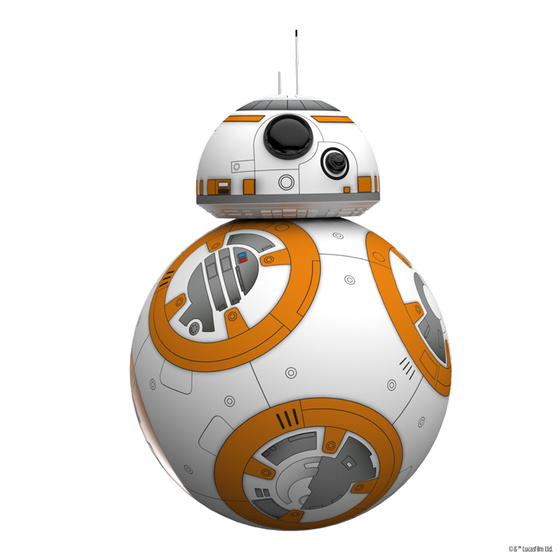
\includegraphics[scale=0.06]{robot}};
      \fill (1,-2) rectangle (2,2); \\
	   % \pgfmatrixnextcell
    }
\end{tikzpicture}
\caption{Exemple d'applications pour robots mobiles}
\label{fig:port:resume}
\end{figure}
Ils doivent se coordonner pour contrôler des
% tenir éloignés les voleurs des
conteneurs de marchandises, en vérifiant régulièrement qu'aucun d'eux
n'a été ouvert. Si un intrus est repéré, les robots doivent le
repousser à l'extérieur du périmètre de sécurité, puis retourner
surveiller les conteneurs. 

Un système constitué d'une telle équipe est appelé \emph{système
  distribué} ou \emph{réparti} \cite{Lynch96,Tel:2001:IDA:517021}. Ce
qualificatif de ``distribué'' provient du fait que le système est
composé d'un ensemble d'entités de calcul autonomes dotés de capacités
de communication qui leur permettent de résoudre une tâche commune.
Traditionnellement, les entités sont immobiles et communiquent les
unes avec les autres par passage de messages.  Le modèle de robot que
nous étudions dans cette thèse diffère du modèle classique par deux
aspects: les entités sont mobiles et ne communiquent pas par passage
de messages. Par ailleurs, ces entités mobiles peuvent être dotés de
capacités limitées.

Les travaux menés sur les réseaux de robots mobiles s'intéressent aux
caractéristiques de bases qui sont nécessaires afin que l'équipe de
robots puisse accomplir une tâche donnée, en l'absence de toute
autorité centrale. Ces travaux considèrent des déplacements des robots
dans un plan euclidien ou dans un environnement discret.  Les tâches
données peuvent être critiques, il faut donc veiller à ce que les
robots les accomplissent correctement, en dépit de leurs limitations.

Jusqu'à présent, les réseaux de robots ont été étudiés de manière
empirique et la plupart des résultats ont été validés seulement par
des preuves faites ``à la main''. Ces preuves visent à vérifier que
l'objectif des robots, appelé \emph{spécification} du problème et
décrit par un ensemble de propriétés, est satisfait. Elles sont
difficiles à lire et à écrire, car le raisonnement sur des systèmes
complexes est à la fois lourd et source d'erreurs.  L'utilisation de
preuves automatiques, basées sur un modèle mathématique abstrait du
système, pourrait simplifier ce processus de vérification. Pour ces
techniques de vérification formelle, plusieurs approches existent :
\begin{itemize}
\item La \emph{génération automatique de tests} prend en entrée
  une description formelle des comportements souhaités du système et
  génère un ensemble de tests à effectuer, qui doit couvrir un
  ensemble de comportements le plus grand possible. Le système est
  ensuite exécuté conformément à ces tests, et l'on peut vérifier si
  les sorties sont identiques à celles attendues.  Cependant il n’est
  pas toujours possible de fournir un ensemble exhaustif de tests, et
  la conception de tests est difficile pour les systèmes concurrents
  ou distribués.
%
\item La \emph{démonstration automatique} laisse l’ordinateur prouver
  automatiquement des théorèmes décrivant les propriétés du système,
  en se basant sur une description mathématique du programme, et sur
  un ensemble de règles de déduction et d’axiomes.  Cette méthode
  n’est cependant pas totalement automatisable, et l’assistant de
  preuves a besoin d’être plus ou moins guidé par une aide humaine
  pendant le processus. D'ailleurs, quand une preuve échoue, il est
  difficile d'en connaitre la raison. Divers assistants de preuve ont
  émergé depuis les années 60, par exemple PVS
  \footnote{http://pvs.csl.sri.com}, Coq
  \footnote{https://coq.inria.fr/} et Isabelle/HOL \footnote{https:
    //isabelle.in.tum.de} sont parmi les plus largement utilisés.
\item Le \emph{model-checking} part d’une représentation abstraite (un
  \emph{modèle}) du programme et d’une spécification formelle des
  comportements souhaités, et vérifie de façon exhaustive et
  automatique que tous les comportements du modèle satisfont cette
  spécification. Bien sûr, la recherche n’est exhaustive que sur
  l’abstraction du système considérée.  Un avantage de cette technique
  est sa complétude et sa capacité à extraire des comportements
  invalidant les propriétés. Ainsi, le \emph{model-checking} peut être
  utilisé dès la phase de conception pour valider les prototypes du
  système. L'explosion combinatoire est l'inconvénient majeur de cette
  méthode : explorer symboliquement toutes les exécutions (l'ensemble
  peut être infini) dans un modèle de grande taille est très
  consommateur de temps et de mémoire. Les
  models-checkers \textsc{Uppaal} \footnote{http://www.uppaal.org} et
  \textsc{Spin} \footnote{http://spinroot.com/spin/whatispin.html}
  sont parmi les plus connus.
\end{itemize}
Chacune de ces approches a ses avantages et ses inconvénients : alors
que les tests peuvent être faciles à mettre en œuvre, ils ne peuvent
pas être appliqués dans la phase de conception, et la génération de
tests exhaustifs est difficile.  Les preuves sont difficiles à mettre
en œuvre car elles nécessitent la présence d'un expert, mais elles
sont exhaustives, applicables dés la phase de conception, et peuvent
s'appliquer à des systèmes dits \emph{paramétrés}, où certaines
variables ne sont pas spécifiées, comme par exemple le nombre de
processus. Enfin, le \emph{model checking} est une approche globale et
automatique, mais limitée par la taille du modèle.  En outre, le
problème du \emph{model checking} de systèmes paramétrés est
indécidable en général~\cite{apt.kozen.86}.

Alors que le \emph{model checking} vérifie qu'un modèle satisfait une
propriété, la \emph{synthèse} consiste à se donner une spécification
et à générer, si possible, un modèle qui la satisfasse. 
% mise en oeuvre à la fin du processus de création d'un algorithme, 
% on souhaite que les méthodes formelles apparaissent au début du processus 
% de création.  La synthèse automatique d'algorithmes est une méthode
%formelle qui permet de générer un algorithme à partir de sa
%specification. 
L'avantage de cette méthode est qu'elle se situe en amont de la
conception et que les protocoles ainsi générés sont corrects par
construction.  Les premiers travaux sur la synthèse remontent à
Church~\cite{Church62} et ont été développés ensuite
dans~\cite{BuchiLandweber69,emersonclarke1981,
  MannaWolper84,PnueliR90}.
%It is even more difficult when the program to generate is intended 
%to work as an open system, maintaining an on-going interaction 
%with a (partially) unknown environment. 
Formellement, le problème de décision est le suivant : étant donnée
une spécification, existe-t-il un modèle qui la satisfasse ? Le
problème de synthèse proprement dit consiste, lorsque la réponse est
positive, à construire effectivement le modèle.

Dans le cas de systèmes ouverts, qui interagissent avec un
environnement, Buchi et Landweber \cite{BuchiLandweber69} ont montré
que le problème était décidable dans le cadre de la théorie des jeux.
Cette approche consiste à considérer le problème de synthèse comme un
\emph{jeu} entre le système et l'environnement. Le système et son
environnement sont deux joueurs qui s'affrontent, et le système gagne
s'il satisfait la spécification initiale. Ainsi, trouver un modèle qui
satisfait la spécification revient à trouver une stratégie gagnante
pour le système, quel que soit les stratéges de l'environnement.
% Ensuite, le
% problème classique en théorie des jeux qui consiste à trouver des
% stratégies gagnantes pour les joueurs est équivalent à trouver comment
% le système doit agir dans toutes les situations, afin de toujours
% satisfaire ses spécifications. 
Toutefois, ce problème est aussi indécidable en général pour les
systèmes distribués, la décidabilité étant obtenue avec des
hypothèses supplémentaires sur l'architecture~\cite{PnueliR90}.

Dans ce travail, notre objectif est d'étudier comment les méthodes
formelles peuvent être appliquées dans le contexte d'algorithmes de
robots mobiles.  Après une présentation de ces algorithmes, nous
montrons les avantages de ces méthodes par rapport aux approches
traditionnelles.



\section{Robots Mobiles}
Dans cette thèse nous nous sommes intéressés à un modèle théorique
\cite{suzuki_distributed_1999,FPS12} dans lequel les robots qui
coopèrent pour atteindre un objectif commun ont des capacités
limitées.  Les robots fonctionnent selon un cycle composé de trois
phases: \emph{Look, Compute} et \emph{Move}. Quand un robot exécute la
première phase, il examine l'environnement qui l'entoure et s'inscrit
dans un repère constitué par l'ensemble des autres robots. Dans la
deuxième phase, il calcule un futur mouvement en fonction de sa
position relative aux autres robots, et enfin, dans la dernière phase,
il met en \oe{}uvre le mouvement calculé précédemment.
 
Ce modèle, appelé SYm (ou ATOM), correspond à un comportement
synchrone des robots, qui exécutent ensemble chacune des
phases. Il a été étendu par Prencipe~\cite{prencipe_new_2000} afin
de prendre en compte un comportement asynchrone plus réaliste pour des
systèmes distribués. Ce nouveau modèle porte le nom de CORDA.  Ces
modèles diffèrent par leurs degrés d'atomicité:
\begin{itemize}
\item Dans le modèle historique, ATOM \cite{suzuki_distributed_1999},
  un sous ensemble de robots exécute chacune des trois phases de manière
  atomique. Il existe deux variantes : Fsync (Fully-synchronous) où tous
  les robots sont synchronisés, et Ssync (Semi-synchronous) où à
  chaque cycle, seul un sous-ensemble de robots s'exécute de manière
  synchrone.

  Dans ce modèle, le comportement du système correspond à l'exécution
  de toutes les opérations instantanément, la conséquence est qu'aucun
  robot ne pourra jamais être observé alors qu'il se déplace, et la
  compréhension de l'univers par les robots actifs est toujours
  cohérente.
\item Le second modèle, CORDA~\cite{prencipe_new_2000} ou Async, est
  une variante moins contrain\-te et donc plus réaliste, où chaque robot
  peut être activé de manière asynchrone, indépendamment des autres
  robots. La durée de chaque phase, et le temps entre les phases
  successives d'un même cycle sont limitées mais inconnues. En
  conséquence, les calculs peuvent être basés sur des observations
  totalement obsolètes, prises arbitrairement loin dans le passé.
\end{itemize}
Notons qu'en terme d'exécutions, Fsync est inclus dans Ssync et Ssync
est inclus dans Async.  \bigskip

La capacité d'une équipe à réaliser une tâche assignée dépend
principalement de ses membres et de leurs capacités: plus les robots
sont puissants, plus le problème est résolu facilement. Les robots du
modèle considéré ici disposent quant à eux de capacités très limitées.
Nous allons maintenant détailler les hypothèses minimales généralement
faites sur les capacités de ces robots.
 
%They are endowed with sensing, computing, 
%and moving capabilities described below. 
\subsection{Des robots restreints}
%Anonymous and similar: 
Les robots sont identiques et anonymes, ils exécutent le même
algorithme et ils ne peuvent pas être distingués par leur apparence,
mais ils peuvent avoir des vitesses de calcul et de déplacement
différentes (dans le cas asynchrone). De plus ces robots peuvent avoir
des identités mais ni eux ni les autres robots n'ont connaissance ou
accès à ces identités.

%oblivious
Les robots sont amnésiques \ie ils n'ont aucun souvenir de leurs
actions
passées. % de leurs actions ne dépendent pas des actions précédentes.
Cette carctéristique implique que tout état peut être considéré comme
initial. Par conséquent, les algorithmes de robots sont
auto-stabilisants : un algorithme distribué est dit \emph{auto-stabilisant}
s'il assure qu'un comportement correct peut être retrouvé en un temps
fini sans aucune aide exterieure.
%In~\cite{DieudonneP12}, Dieudonne et Petit discuss 
%on the link between the mobile robot model and self-stabilization.

%no common handedness: 
Les robots n'ont pas un sens commun de l'orientation.  Chaque robot a
sa propre unité de longueur, et possède une boussole locale
définissant son propre système de coordonnées cartésiennes locales. Ce
système de coordonnées local est auto-centré, \ie l'origine est la
position du robot. De plus, le système de coordonnées local des robots
peut complètement changer à chaque cycle, mais il reste invariant au
cours d'un cycle.

%no communication; other works communication: via msg, pebbles, ...
Les robots sont silencieux : il ne communiquent pas entre eux de
manière explicite, mais seulement en observant les positions des
autres robots, et prennent leurs décisions en conséquence. En d'autres
termes, le seul moyen pour un robot d'envoyer des informations à un
autre robot est de se déplacer et de laisser les autres robots
observer son mouvement avant de bouger à nouveau.

Bien que dans la littérature des robots plus faibles soient étudiés,
nous nous sommes intéressés dans cette thèse aux robots décrit par le
modèle original de Suzuki et Yamashita \cite{suzuki_distributed_1999}.

\subsection{Les capacités des robots}
Pour exécuter leurs cycles Look-Compute-Move, les robots peuvent
observer leur environnement, prendre des décision et se mouvoir.  Deux
types d'environnements ont été étudiés :
\begin{itemize}
\item  le plan euclidien (continu) \cite{suzuki_distributed_1999,FPS12},
%dans lequel les robots évoluent dans le plan; 
\item un environnement
  discret~\cite{KlasingMP06,flocchini_computing_2007}, représenté par
  un graphe, dans lequel les noeuds correspondent aux différentes
  positions possibles et les arcs aux routes permettant aux robots
  d'aller d'une position à une autre.
\end{itemize}
La représentation discrète est motivée par des aspects pratiques liés
au manque de fiabilité des dispositifs d'observation utilisés par les
robots ainsi qu'à l'imprécision de leur
motorisation~\cite{CDDMJ08j}. Cela permet notamment de simplifier la
conception des modèles en raisonnant sur des structures
finies. Cependant, ce cadre rend le modèle plus sensible à
la taille des constantes, ce qui peut augmenter de manière
significative le nombre de configurations symétriques lorsque le
graphe sous-jacent est également symétrique (par exemple un anneau) et
donc la taille des preuves de correction~\cite{ASN11c, KLOT11,
  KLOT12}.

\subsubsection{Observation}
\index{Visibility} Les robots sont dotés de capteurs de vision
fournissant les emplacements des autres robots. L'emplacementCette
information est obtenue soit avec un grain fin (donc un certain degré
de précision), soit avec un grain. Dans le premier cas, la littérature
se réfère principalement au modèle où l'espace est continu, tandis que
dans le second cas l'environnement est discret.

Les robots n'ont pas de dimension et donc leur visibilité ne peut être
obstruée: si trois robots $r_1$, $r_2$, et $r_3$ sont alignés, avec
$r_2$ au milieu, $r_1$ peut quand même voir $r_3 $. Les robots peuvent
théoriquement partager la même position : cette formation est appelée
une \emph{tour} \cite{FPS12}. La capacité pour un robot de détecter la
multiplicité est essentielle pour réaliser certaines tâches
particulières. Parmi les détecteurs de multiplicité, nous distinguons :

\begin{itemize}
\item les détecteurs \emph{faibles}, capables de déterminer s'il y a
  zéro, un ou plusieurs robots à une position particulière,
\item les détecteurs  \emph{forts} qui fournissent le nombre exact
  de robots à une position particulière.
\end{itemize}
Le capteur correspondant peut être local ou global : dans le contexte
local un robot ne détecte que la multiplicité à sa position courante,
alors que dans le cadre global le nombre de robots sur chaque position
est connu.  Dans le modèle que nous étudions il n'y a aucune
restriction sur la distance de visibilité des robots.

\subsubsection{Calcul}
Comme dans les systèmes distribués classiques, les robots sont
supposés être en mesure d'effectuer toute suite finie de calculs en
temps négligeable. Comme les robots sont amnésiques, la mémoire
volatile est utilisée pour effectuer le cycle Look-Compute-Move, le
contenu de la mémoire est effacé à la fin de chaque cycle.  Le calcul
prend en entrée l'observation faite dans la phase Look et retourne un
movement.  Lorsque deux robots sont sur la même position ou sont
symétriques, ils calculent le même mouvement.

\subsubsection{Mouvement}
Les robots peuvent se déplacer seulement à l'emplacement déterminé par
la phase de calcul du cycle en cours. Dans certains cas, en raison de
la symétrie, la position calculée peut être ambiguë : elle correspond
alors à un mouvement non déterministe, qui peut être résolu par un
ordonnanceur. Dans le modèle discret, un robot peut se déplacer
seulement vers un emplacement adjacent à sa position
courante. Dans le modèle continu, un robot se déplace vers sa
destination quelle qu'elle soit.

%schedulers %%%%%%%%%%%%%%fairness%%%%%%%%%%%%
\subsubsection{Ordonnancement}
\index{Fairness} Lorsque plusieurs processus veulent s'exécuter
simultanément, il est nécessaire de determiner lequel sera exécuté et
à quel moment.  Les ordonnanceurs sont des abstractions utilisées pour
caractériser le degré d'asynchronisme des
robots~\cite{DefagoGMP06,FPS12}.  Un ordonnanceur \emph{équitable} est
généralement utilisé, il active tous les robots infiniment souvent,
%afin d'éviter la famine, 
mais certains robots peuvent être activés
arbitrairement plus que les autres.

Il existe d'autres types d'équité qui dépendent de l'ordonnancement
des actions plutôt que des processus.  Un ordonnanceur \emph{fort}
garantit que chaque action tirable infiniment souvent possible sera
exécutée infiniment souvent. Un ordonnanceur \emph{faible} garantit
que chaque action tirable continûment à partir d'un certain moment
sera exécutée une infinité de fois.
 

\bigskip Dans cette thèse, nous considérons des robots dans un univers
discret.  Nous nous sommes principalement intéressés à deux problèmes
largement étudiés pour les robots mobiles et autonomes : le premier
est celui du rassemblement \cite{markoubook}, où les robots doivent se
retrouver sur une unique position, le second est celui de
l'exploration \cite{flocchini_computing_2007,
  devismes_optimal_2010-1}, où les robots doivent visiter tous les
noeuds du graphe.

Le problème du rassemblement est le premier à avoir été étudié dans la
littérature, aussi bien
historiquement~\cite{suzuki_distributed_1999,KlasingMP06,
  klasing_taking_2008,Pelc11} que par le nombre de publications.
Quelles que soient leurs positions initiales, les robots doivent se
déplacer afin d'être finalement tous regroupés sur une même position,
non connue à l'avance, et y rester par la suite.  Comme le problème de
consensus dans les systèmes distribués classiques, où toutes les
entités doivent se mettre d'accord sur une même valeur, le
rassemblement a une définition simple, mais l'existence d'une solution
dépend du degré de synchronisme du système.

Un équipe de robot a exploré un graphe si chaque position de celui-ci
est visité par au moins un robot.  Le problème de l'exploration a
plusieurs variantes, parmi lesquelles nous avons étudié l'exploration avec
arrêt et l'exploration perpétuelle exclusive.  L'exploration avec
arrêt est la version historique du travail sur l'exploration
\cite{flocchini_computing_2007,lamani_optimal_2010,devismes_optimal_2010-1}.
Les robots doivent atteindre une configuration dans laquelle ils sont
tous inactifs et où chaque noeud du graphe a été visité par au moins
un robot. La difficulté de cette tâche réside dans le fait que les
robots doivent s'arrêter une fois l'exploration faite. En l'absence de
mémoire persistante, cela signifie qu'ils doivent être en mesure de
faire la distinction entre les différentes étapes du processus
d'exploration.  L'exploration perpétuelle exclusive a été étudiée plus
récemment \cite{blin_exclusive_2010, navarraipdps2013}.  Chaque noeud
du graphe doit être visité infiniment souvent et aucun point de
multiplicité ne doit apparaître.
	
%%%%%%%%%%%%%%%%%%%%%%%%%VERIFICATION%%%%%%%%%%%%%%%%%%%%%%%%%%%%%
\section{Méthodes formelles et algorithmes de robots}
L'utilisation de méthodes formelles exige des représentations
mathématiques du système et de sa spécification, donnée comme un
ensemble de propriétés.  Un système distribué est souvent décrit comme
un système de transition \cite{Tel:2001:IDA:517021,
  DBLP:books/mk/Lynch96}, composé des modèles de ses sous-systèmes.
Les propriétés peuvent être classées en différents types, parmi
lesquels les propriétés de sûreté et de vivacité. Les propriétés de
sureté exigent que \og{}quelque chose de mauvais ne se produise
jamais\fg{}, comme l'absence de blocage dans l'exécution d'un système.
Les invariants forment une sous-classe importante des propriétés de
sûreté, exprimant que \og{}quelque chose est vrai à chaque étape de
chaque exécution\fg{}.  Les propriétés de vivacité exigent que
\og{}quelque chose de bon finisse par arriver\fg{}, par exemple que 
% qu'il n'y aura pas de famine, 
chaque processus ait finalement accès aux ressources critiques.  Toute
spécification peut être écrite comme la conjonction de propriétés de
sécurité et de vivacité \cite{AlpernS85}.
		

\subsection{Model-checking}
Un \emph{model-checker} prend en entrée un modèle $M$, souvent sous la
forme d'un système de transitions, décrivant toutes les exécutions
possibles du système, et la propriété à vérifier, exprimée par une
formule logique $\varphi$. Il détermine si le modèle satisfait ou non
la formule. Lorsque la propriété n'est pas satisfaite, le
\emph{model-checker} fournit un contre-exemple, \ie une exécution du
modèle qui invalide la propriété. Ce contre-exemple est utile pour
trouver des erreurs dans les systèmes complexes, c'est un avantage
majeur du model-checking par rapport aux autres méthodes formelles,
comme la démonstration de théorèmes, qui peuvent infirmer une
propriété, mais sans fournir systématiquement un tel contre-exemple.

%\todo{The automata approach}
L'approche par automates pour le \emph{model-checking} a été
introduite par Vardi et Wolper~\cite{vardi_automata-theoretic_1986},
afin de fournir un cadre unifié et extensible, d'abord appliqué à une
classe de formules logiques appelée \textsf{LTL}.  Cette approche
comprend trois étapes :
\begin{itemize}
\item Tout d'abord le système et ses spécifications doivent être
  modélisés. Soit $M$ le modèle du système, et $\varphi$ la formule
  \textsf{LTL} représentant la spécification du système.  Le langage
  $\mathcal{L} (M)$ associé à $M$ représente toutes les exécutions de
  $M$.  La négation de la formule $\varphi$ est traduite en un
  automate $\mathcal{A}_{\neg \varphi}$ dont le langage,
  $\mathcal{L}(A_{\neg \varphi})$, est l'ensemble des exécutions qui
  invalident $\varphi$.
\item Les automates $M$ et $\mathcal{A}_{\neg \varphi}$ sont
  synchronisés afin d'obtenir un automate $M \times \mathcal{A}_{\neg
    \varphi}$ dont le langage $\mathcal{L}(M \times \mathcal{A}_{\neg
    \varphi}) = \mathcal{L} (M) \cap \mathcal{L} (\mathcal{A}_{\neg
    \varphi})$, est l'ensemble des exécutions de $M$ qui invalident
  $\varphi$.
\item Enfin, le \emph{model-checker} effectue un test de vacuité
  sur le produit. Le modèle $M$ satisfait $\varphi$ si et seulement si
  $\mathcal{L} ( M \times \mathcal{A}_{\neg \varphi}) = \emptyset$.
  Si le test de vacuité est positif, cela veut dire qu'aucune
  exécution n'invalide $\varphi$, les propriétés exprimées par
  $\varphi$ sont donc satisfaites par le modèle $M$. Sinon, une
  exécution de $M$ qui invalide $\varphi$ est retournée comme
  contre-exemple.
\end{itemize}		

L'inconvénient de cette méthode est le problème bien connu
d'\emph{explosion combinatoire}~\cite{Valmari96}, lorsque le produit
$M \times \mathcal{A}_{\neg \varphi}$ est de grande taille.  En
particulier, lorsque le modèle $M$ du système est lui-même obtenu par
produit de plusieurs composants, sa taille est exponentielle en le
nombre de processus. Ainsi, dans l'approche par automates, le produit
est souvent trop grand pour que le test de vacuité puisse être réalisé
dans un délai raisonnable en terme de temps d'exécution ou de mémoire
utilisée.

Les systèmes distribués sont naturellement structurés comme un
ensemble de plusieurs processus, parmi lesquels certains présentent
des comportements similaires. De tels composants sont dits
symétriques, et connaître le comportement d'un de ces composants est
souvent suffisant pour connaître le comportement de ses pairs. Plus
formellement, les symétries du système définissent une relation
d'équivalence sur ses états, qui permet de construire un espace
d'états réduit, par quotient, où au moins un état par classe
d'équivalence est maintenu.  Si un seul représentant par classe est
maintenu, la réduction maximale est atteinte. La définition de
symétries garantit que l'espace d'états réduit préserve les
propriétés, si les symétries sont respectés~\cite{ClarkeJEF96,
  EmersonS96}. Cette réduction est généralement exponentiellement plus
petite que l'espace d'états initial, ce qui réduit le temps
d'exécution et la mémoire utilisée lors la procédure de vérification.

À notre connaissance, dans le contexte des réseaux de robots mobiles
opérant dans l'espace discret, une seule tentative, par Devismes
\emph{et al.}~\cite{devismes_optimal_2011}, a étudié la possibilité
d'utiliser le model-checking comme méthode de vérification. Les auteurs
utilisent LUSTRE~\cite{lustre:ieee} pour décrire et vérifier le
problème de l'exploration avec arrêt sur une grille de taille $ 3
\times 3 $, par $3$ robots, dans le modèle Ssync.  Ils considèrent un
type particulier de configurations avec une tour de 2 robots et un
robot isolé, où seul le robot isolé souhaite se déplacer.  Ils
vérifient l'invariant: \emph{nœuds visités} $\leq 4 $, ce qui leur
permet de compléter leurs preuves manuelles par de la vérification
formelle pour ce cas précis.
	
\subsection{Preuves}
En utilisant un assistant de preuves, un utilisateur peut exprimer des
données, des programmes, des théorèmes et des preuves.  Les assistants
de preuves fournissent une garantie supplémentaire en vérifiant
mécaniquement la solidité de la preuve une fois qu'un expert l'a
développée de manière interactive.  Ils ont été utilisés avec succès
pour diverses tâches telles que la formalisation de la sémantique des
langages de programmation \cite{Leroy09}, la certification d'un noyau
de l'OS \cite{KleinAEHCDEEKNSTW10}, ou la vérification de protocoles
cryptographiques \cite{AlmeidaBBBKB12}.  Au cours des vingt dernières
années, l'utilisation d'assistants de preuves automatiques s'est
étendue à la validation de systèmes distribués.

L'inconvénient majeur de cette méthode est qu'elle nécessite un fort
niveau d'expertise pour l'écriture de la preuve. De plus elle n'est
pas complètement automatique, car les preuves sont souvent obtenues à
partir de nombreux lemmes.

Pour le modèle de robots, Courtieu \emph{et al.} ont utilisé COQ afin
de certifier des résultats d'impossibilité, en présence
de processus byzantins \cite{AugerBCTU13}. Une preuve certifiée du
résultat de \cite{suzuki_distributed_1999} est proposé
dans \cite{CourtieuRTU15}, confirmant l'impossibilité de regrouper deux
robots. Les auteurs fournissent également un résultat plus général
d'impossibilité : rassembler un nombre pair de robots, lorsque deux
robots sont initialement sur la même position, est impossible.
		
\subsection{Synthèse d'algorithmes}
%Même s'il est utile de vérifier/ prouver des algorithmes existants,
Les techniques de synthèse sont situées plus en amont, puisqu'elles
permettent, dans certains cas, de générer automatiquement un
algorithme correct.  Pour cela, soit $\varphi$ la spécification que le
système doit satisfaire, et soit $E$ un modèle de l'environnement.  Le
problème de synthèse cherche s'il existe un programme $P$ tel que $P
\times E$ satisfait $\varphi$. Ainsi, le système décrit par $P$atteint
son objectif, quel que soit le comportement de l'environnement.
% la synthèse prend en entrée la
% spécification d'un système interagissant avec un environnement, et
% demande s'il existe un programme qui satisfasse cette spécification,
% quel que soit le comportement de l'environnement.
Lorsque la réponse est positive, le programme doit alors être
construit.  Une réponse négative donne une preuve qu'il y a toujours
une façon pour l'environnement d'empêcher le système d'atteindre son
objectif. Une telle stratégie de l'environnement peut donc être vue
comme une preuve d'impossibilité.

%  Le comportement du système ainsi créé doit
% correspondre exactement à tous les comportements admissibles par la
% spécification.

Au premier abord on pourrait croire que le modèle réellement
nécessaire est celui des \emph{jeux distribués}, dans lequel chaque
robot représente un joueur distinct, tous ces joueurs coopérant contre
un environnement hostile. Dans les jeux distribués, l'existence d'une
stratégie gagnante pour l'équipe de joueurs est indécidable
\cite{PetersonReif79}. Cependant, le fait que les robots soient
capables de voir leur environnement, et donc de toujours connaître la
configuration du système, nous permet de rester dans le cadre de jeux
à deux joueurs. Il est donc possible de coder l'ensemble des robots comme
un seul joueur.  Bien sûr, la stratégie obtenu sera centralisée, le
jeu devra être conçu afin de n'obtenir que des stratégies qui peuvent
être distribuées afin d'être implémentées sur les robots.

À notre connaissance, dans le contexte des réseaux de robots mobiles,
une seule tentative \cite{BDPPT12c} examine la possibilité de
synthétiser automatiquement des protocoles de robots mobiles.  Ce
travail considère l'exploration perpétuelle exclusive par $k$ robots
d'anneaux de tailles $n$ quelconque dans le modèle Ssync.  L'approche
choisie est \emph{brute force} : tous les protocoles possibles sont générés
mécaniquement sans qu'aucune propriété à satisfaire ne soit
spécifiée. Les protocoles ainsi obtenus ne contiennent aucune
\emph{ambiguïté}, c'est à dire qu'ils ne contiennent pas de
configurations symétriques, ni de de multiplicité.  Une fois ces
protocoles construits chacun est étudié manuellement afin de voir s'il
permet ou non une exploration perpétuelle exclusive. Tous les
protocoles qui le permettent sont ensuite comparés afin d'obtenir une
étude qualitative.

Dans cette thèse nous avons voulu donner suite à ces travaux, en
démontrant que le model-checking pouvait être utilisé dans les réseaux
de robots afin de vérifier des instances de protocoles entiers et non
seulement comme aide pour des preuves manuelles.  Nous avons voulu
également montrer le pouvoir de la synthèse qui permet de générer
automatiquement des algorithmes corrects par construction sans se
restreindre sur les mouvements ou les configurations possibles.  Notre
approche diffère des précédentes, car notre modèle est suffisamment
général pour décrire tous les modèles d'atomicité, alors que les
travaux antérieurs ne gèrent que les modèles synchrones.



\section{Contributions}
		%\todo{model}
Nous proposons un modèle formel représentant un réseau de robots
mobiles comme un produit d'automates.  Ce modèle permet de décrire les
trois hypothèses d'exécution décrites ci-dessus, à savoir Fsync, Ssync
et Async. Nous en réalisons une implémentation qui permet de réduire
la taille de l'espace d'états en utilisant les symétries du modèles.

Grâce à ce modèle, nous produisons deux contributions, relatives à la
vérification et à la synthèse.

\paragraph{Vérification.} Nous avons tout d'abord vérifié formellement
certaines instances de deux protocoles existants, qui permettent de
résoudre les deux variantes de l'exploration d'anneau avec des robots
asynchrones.  Afin de vérifier les algorithmes de robots évoluant sur
un anneau, nous avons créé un générateur de modèles qui,
indépendamment de la tâche à effectuer, prend en entrée la taille de
l'anneau, le nombre de robots, le modèle d'exécution du système et un
algorithme à vérifier sous la forme de transitions gardées, puis
construit le modèle du système. Une fois les spécifications du système
formellement énoncées, l'utilisation d'un model-checker nous permet de
vérifier l'algorithme pour une taille d'anneau et un nombre de robots
fixés.  Nous avons d'abord vérifié le protocole de Flocchini \emph{et
  al} qui résout le problème de l'exploration avec arrêt \cite{
  flocchini_computing_2007}, puis nous avons étudié le problème de
l'exploration perpétuelle exclusive avec l'algorithme de Blin \emph{et
  al} \cite{blin_exclusive_2010}. Dans les travaux d'origines, les
deux protocoles ont été donnés par une suite de descriptions
informelles, que nous avons dû formaliser.

$\bullet$ Dans le cas de l'exploration avec arrêt
\cite{flocchini_computing_2007}, l'algorithme a été prouvé correct
grâce à une preuve manuelle lorsque le nombre de robots est $k > 17 $
et $ n $ (la taille de l'anneau) et $ k $ sont premiers entre eux.  La
nécessité de la borne $k > 17 $ n'ayant pas été prouvée dans le papier
d'origine, notre méthodologie démontre que pour de nombreux cas de $k
$ et $ n $ non couverts dans le document original, le protocole est
toujours correct. Nous proposons une conjecture pour les cas avec $ k
\leq 17 $ robots.
 
$\bullet$ Nous avons ensuite étudié l'algorithme de Blin \emph{et al } qui
permet à un nombre minimal de $3$ robots d'explorer perpétuellement un
anneau sans que des collisions ne surviennent
\cite{blin_exclusive_2010}.  Dans ce cas, notre méthodologie a permis
d'obtenir un contre-exemple relevant d'un défaut subtil dans
l'algorithme, lorsque celui est exécuté dans le modèle asynchrone.
Nous proposons une correction du protocole original et vérifions par
\emph{model-checking} plusieurs instances du nouvel algorithme. Nous
terminons cette étude en donnant une preuve inductive de ce protocole
pour des anneaux de tailles quelconques.

\paragraph{Synthèse.} La deuxième contribution de cette thèse porte
sur la synthèse automatique de protocoles pour les réseaux de robots.
Notre but est de montrer comment réaliser la synthèse de protocoles de
rassemblement pour des robots évoluant dans un environnement discret.
Nous avons examiné séparément les modèles synchrones et asynchrones.

$\bullet$ Nous avons d'abord proposé un encodage du problème de
rassemblement par un jeu d'accessibilité avec deux joueurs : la
coalition de robot d'une part et son adversaire, qui est
l'ordonnanceur. L'adversaire décide également le sens de déplacement
des robots désorientés, à chaque activation. Notre encodage est assez
expressif pour englober les deux modèles synchrone Ssync et Fsync, y
compris lorsque plusieurs robots sont situés sur le même noeud et
lorsque des situations symétriques se produisent, contrairement à la
solution ad-hoc de \cite{BDPPT12c}.  Cela nous a permis de générer
automatiquement un algorithme distribué \emph{optimal}, pour trois
robots évoluant sur des anneaux de tailles fixes. Notre critère
d'optimalité se réfère au nombre de mouvements nécessaires pour que
les robots se regroupent.  En étudiant les solutions produites par
l'outil, nous avons pu extraire un \emph{motif}, et en déduire un
algorithme paramètré. Une preuve par induction nous a permis de
prouver que cet algorithme est correct pour toute taille d'anneau dans
le modèle synchrone mais aussi dans le modèle asynchrone.

$\bullet$ Dans le cas asynchrone, nous montrons comment la recherche
d'un algorithme de rassemblement de robots peut être vu comme un jeu à
deux joueurs avec information partielle.  Dans ce type de jeux,
contrairement aux précédents, les joueurs ont une vue incomplète du
système.  Afin de lutter contre l'explosion combinatoire due au modèle
asynchrone, nous proposons un algorithme récursif qui permet d'obtenir
un protocole de rassemblement, en combinant la synthèse d'algorithmes
dans le modèle synchrone avec le \emph{model checking} des solutions
produites, exacutées dans un modèle asynchrone.

	
	
